\chapter{Planificación}

\section{Planificación a priori}

Se trata de planificar como se espera desarrollar el proyecto en el tiempo, para ello se va a hacer uso de un diagrama de Gantt donde se va a proporcionar una vista general de las tareas programadas, estas tareas tendrán que completarse en unas fechas estipuladas.

\subsection{Diagrama de Gantt}

Un diagrama de Gantt es una herramienta útil para planificar proyectos. Proporciona una vista general de las tareas programadas, indicando el periodo de tiempo que tienen para completarse.\\

El diagrama se mostrará:
\begin{itemize}
    \item Fecha de inicio y finalización del proyecto.
    \item Las tareas del proyecto.
    \item Fecha de programada de cada tarea, tanto la de inicio como la de final.
    \item Como se superponen las tareas y si hay relación entre ellas.
\end{itemize}

Con esta planificación se conseguirá una mayor claridad en las tareas a realizar y una mejor gestión del tiempo.

\subsection{Etapas de desarrollo}

\begin{itemize}
    \item \textbf{1ª etapa}: Revisar frameworks para IoT.
    \item \textbf{2ª etapa}: Desarrollar aplicación para IoT.
    \item \textbf{3ª etapa}: Explotación de una vulnerabilidad.
    \item \textbf{4ª etapa}: Documentación.
\end{itemize}

\subsection{Temporización}

De los 3 meses y medios a que se van a dedicar al proyecto, en todos ellos se va a desarrollar las etapas indicadas anteriormente. Se muestra la fecha de inicio y de fin de cada etapa.

\renewcommand{\arraystretch}{1.5}\label{presupuesto-section}
\begin{table}[H]
	\centering
	\label{tabla-temporal}
	\resizebox{\textwidth}{!}{%
	\begin{tabular}{@{}ccc@{}}
		\toprule
		\rowcolor[HTML]{ECF4FF} 
		\textbf{Etapas del desarrollo}                                                                                                                  & \textbf{Fecha de comienzo} & \textbf{Fecha de finalización} \\ \midrule
		\cellcolor[HTML]{ECF4FF}\textbf{\begin{tabular}[c]{@{}c@{}}Documentación del proyecto\end{tabular}} & 9 de Marzo                & 23 de Junio                     \\
		\rowcolor[HTML]{EFEFEF} 
		\cellcolor[HTML]{ECF4FF}\textbf{Revisar frameworks IoT}                                                                                & 21 de Marzo                 & 6 de Abril                    \\
		\cellcolor[HTML]{ECF4FF}\textbf{\begin{tabular}[c]{@{}c@{}}Desarrollar aplicación para IoT\end{tabular}}         & 7 de Abril                & 12 de Mayo                    \\
		\rowcolor[HTML]{EFEFEF} 
		\cellcolor[HTML]{ECF4FF}\textbf{Explotar vulnerabilidad}                                                                                   & 13 de Mayo                & 22 de Junio                     \\ \bottomrule
	\end{tabular}}
	\caption{Organización temporal del proyecto.}
\end{table}

\begin{figure}[ht!]
    \centering
    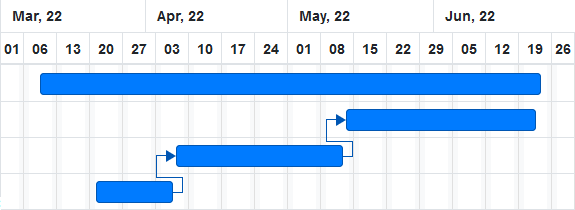
\includegraphics[width=\linewidth]{imagenes/diagramaGantt_v2.png}
    \caption{Diagrama de Gantt. Gráfico.}
    \label{fig:figure3}
\end{figure}

Este gráfico corresponde con la duración de cada etapa, comenzando con la documentación. También se indica que hay etapas que para que estas se puedan empezar a desarrollar necesitan que la anterior este terminada, es el caso de la etapa de \textit{Desarrollo de la aplicación} y de \textit{Explotación de una vulnerabilidad}.

\subsection{Seguimiento del desarrollo}

Con el fin de facilitar la visualización del progreso del proyecto se usan distintas herramientas.

\subsubsection{Trello}

Permite gestionar proyectos de forma sencilla y muy visual. Por cada proyecto se crea un tablero donde podemos crear listas y cada lista almacenará \textit{tarjetas} donde se describirá una tarea u objetivo a cumplir. En nuestro caso el tablero se divide en 7 listas:

\begin{itemize}
    \item \textbf{Dudas}, se dejan ancladas preguntas a los tutores.
    \item \textbf{Objetivos}, para recordar los objetivos que se tienen que completar para el proyecto.
    \item \textbf{Pendientes}, tareas que se tienen que realizar pero no se están desarrollando.
    \item \textbf{En proceso}, tareas que se están trabajando.
    \item \textbf{Pendientes de revisión}, tareas finalizadas que requieren de revisión por parte de los tutores.
    \item \textbf{Terminadas}, tareas que han sido aceptadas en la revisión.
    \item \textbf{Hitos}, se agrupan tareas que forman parte de una misma etapa.
\end{itemize}

\subsubsection{Github}

Se ha creado un repositorio \footnote{Enlace al repositorio: https://github.com/LuisArostegui/TFG} donde se van añadiendo \textit{issues} por cada tarea que se tenga que realizar. Esta tarea es la misma que nos encontramos en el tablero de Trello, por tanto, cuando se crea una nueva tarea en Trello, creamos un nuevo issue con el mismo nombre y descripción para seguir un progreso coherente.\\

También se crean \textit{Milestones} que se corresponde con el nombre y descripción de la lista de \textit{Hitos} del tablero de Trello.\\

Cada vez que terminemos de trabajar en un \textit{Milestone} se creará un \textit{Pull Request} para que los tutores puedan revisar los cambios del proyecto y aceptarlos o rechazarlos. Cada acción que se realice tanto en Trello como en Github se verá reflejado en ambos, de esta manera conseguimos un desarrollo del proyecto realista de principio a final.

\subsubsection{Clockify}

Esta herramienta nos permite seguir el tiempo que estamos trabajando. Cada vez que nos pongamos a trabajar, iniciaremos el contador y nombraremos a ese contador con el nombre de la tarea que estemos realizando en ese momento.

\section{Planificación a posteriori}

Una vez terminado el proyecto nos apoyamos en las distintas herramientas que usamos en la planificación a priori para ver el resultado final. \\

Usando la herramienta de ``Insights`` de Github obtenemos los siguientes resultados:


\begin{figure}[hb!]
    \centering
    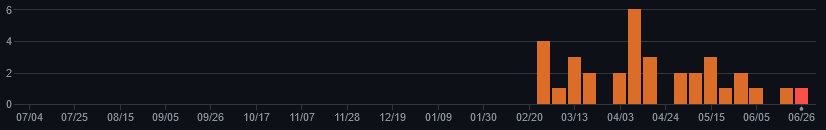
\includegraphics[width=\linewidth]{imagenes/commits.png}
    \caption{Commits realizados por fecha}
    \label{fig:figure4-plan}
\end{figure}

\begin{figure}[hb!]
    \centering
    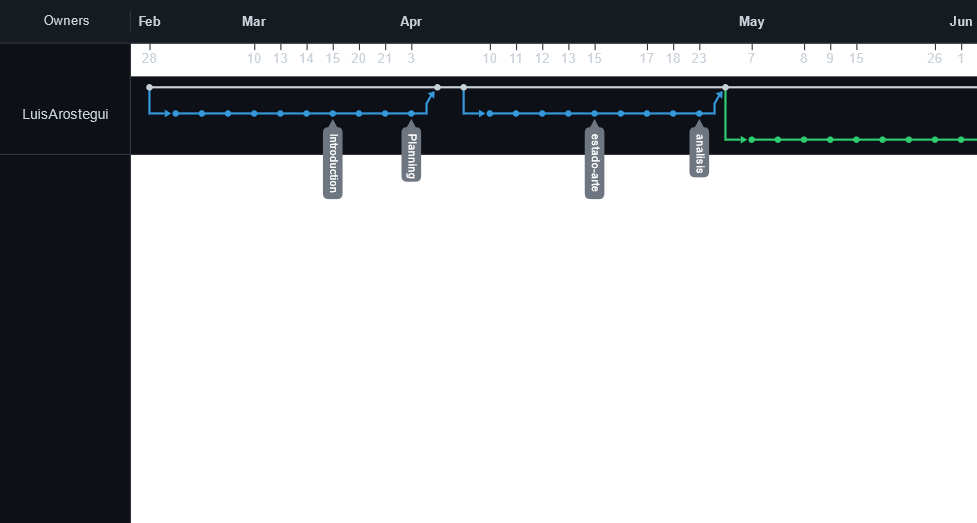
\includegraphics[width=\linewidth]{imagenes/canvas.png}
    \caption{Ramas creadas y forks. Primera parte}
    \label{fig:figure5-plan}
\end{figure}

\begin{figure}[ht!]
    \centering
    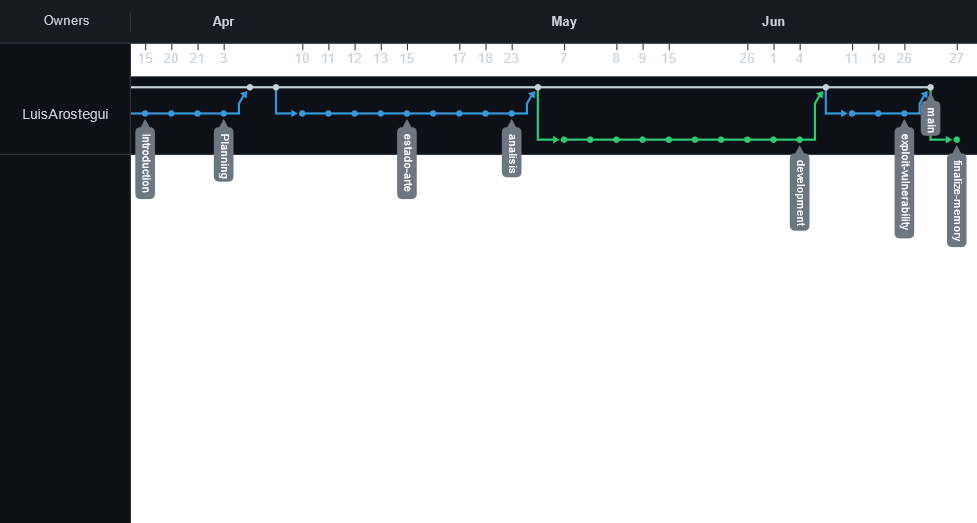
\includegraphics[width=\linewidth]{imagenes/canvas2.png}
    \caption{Ramas creadas y forks. Segunda parte}
    \label{fig:figure6-plan}
\end{figure}

Se empezó a trabajar en Marzo, tal y como se indicó en la planificación pero la finalización del primer objetivo se retrasó hasta el 24 de Abril, pero esto se debe a que se realizó un estudio del paradigma IoT y se fue implementando antes la introducción y sección de estado del arte para hacer un trabajo más completo en el primer objetivo. El desarrollo terminó el 5 de Junio y la explotación de la vulnerabilidad y toda su documentación correspondiente el 26 de Junio. En total se ha retrasado 4 días más de lo previsto. \\

\newpage

Por parte de Trello, nos encontramos que conforme se iba avanzando con el proyecto se han creado tarjetas que se correspondían con Milestones o con issues, el resultado es el siguiente:

\begin{figure}[hb!]
    \centering
    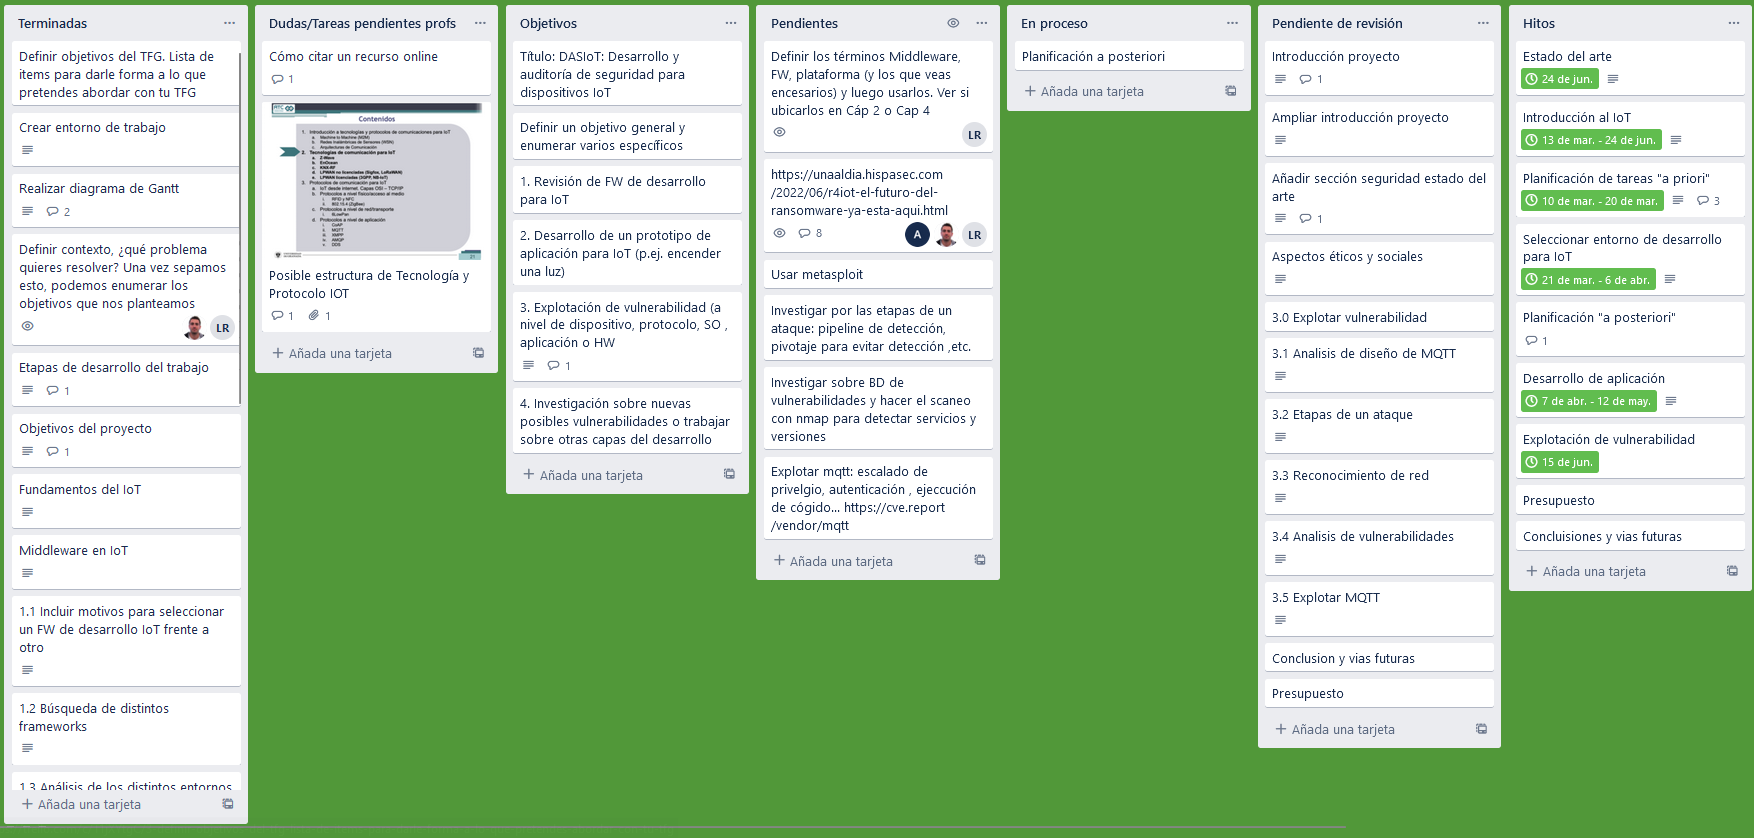
\includegraphics[width=\linewidth]{imagenes/trello.png}
    \caption{Tarjetas creadas en el proyecto en Trello}
    \label{fig:figure7-plan}
\end{figure}

\newpage

Y en clockify este es el seguimiento del tiempo dedicado a cada tarea (correspondiente a la tarjeta de Trello):


\begin{figure}[hb!]
    \centering
    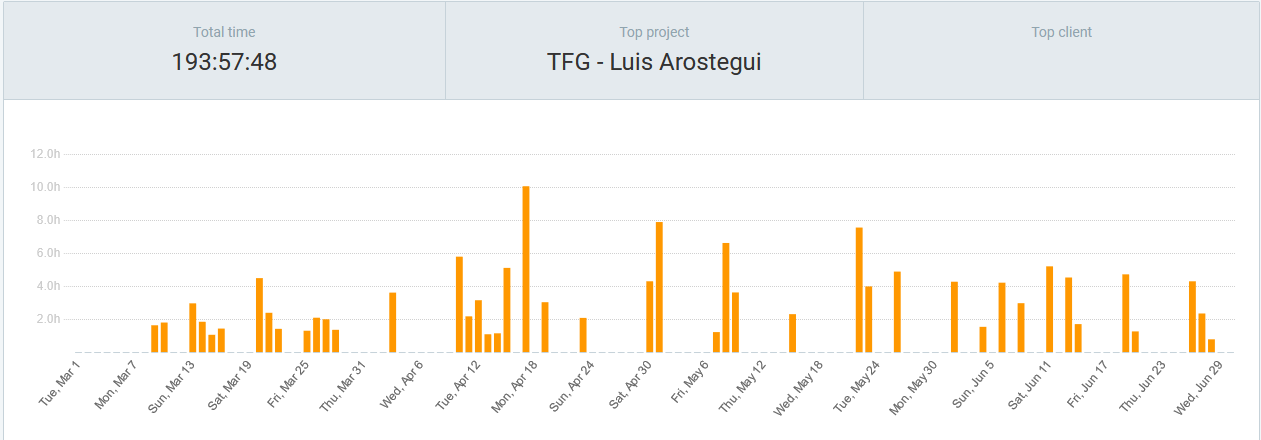
\includegraphics[width=\linewidth]{imagenes/clockify.png}
    \caption{Tiempo dedicado. Clockify.}
    \label{fig:figure8-plan}
\end{figure}




\chapter{Presupuesto}

En una situación donde estemos contratados por una entidad que requiera de nuestros servicios para la auditoría de seguridad de dispositivos IoT, que requiera de la investigación y análisis del paradigma IoT. Teniendo en cuenta que al ser un ingeniero informático sin experiencia laboral, trabajando 5 horas al día, durante 5 días a la semana, un total de 300 horas en 3 meses. Para calcular el precio de la mano de obra, se tiene en cuenta lo que suele cobrar un ingeniero informático sin experiencia, unos 22 mil euros al año a jornada completa, esto se ve reflejado en 6.12€ a la hora, lo que hace un total de 1836€. \\

Una vez vista la mano de obra se ve el coste de los materiales.

\renewcommand{\arraystretch}{1.5}\label{time-section}
\begin{table}[H]
	\centering
	\label{tabla-presupuesto}
	\resizebox{\textwidth}{!}{%
	\begin{tabular}{@{}ccc@{}}
		\toprule
		\rowcolor[HTML]{ECF4FF} 
		\textbf{Descripción}                                                                                                                  & \textbf{Importe por unidad} & \textbf{Total} \\ \midrule
		\cellcolor[HTML]{ECF4FF}\textbf{\begin{tabular}[c]{@{}c@{}}Mano de obra\end{tabular}} & 1836€                & 1836€                     \\
		\rowcolor[HTML]{EFEFEF} 
		\cellcolor[HTML]{ECF4FF}\textbf{Ordenador de sobremesa para desarrollo}                                                                                & 1600€                 & 1600€                    \\
		\rowcolor[HTML]{EFEFEF} 
		\cellcolor[HTML]{ECF4FF}\textbf{Raspberry PI}                                                                                & 40€                 & 40€                    \\
		\cellcolor[HTML]{ECF4FF}\textbf{\begin{tabular}[c]{@{}c@{}}SanDisk Extreme Tarjeta de Memoria microSD de 64 GB\end{tabular}}         & 20€                & 20€                    \\
		\rowcolor[HTML]{EFEFEF} 
		\cellcolor[HTML]{ECF4FF}\textbf{Instalación y mantenimiento de los componentes y software}                                                                                   & 100€                & 100€                     \\
		\cellcolor[HTML]{ECF4FF}\textbf{\textbf{Total completo}}                                                                                   & \textbf{3596€}               &                      \\\bottomrule
	\end{tabular}}
	\caption{Presupuesto total del proyecto.}
\end{table}

